\begin{figure}[h!]
    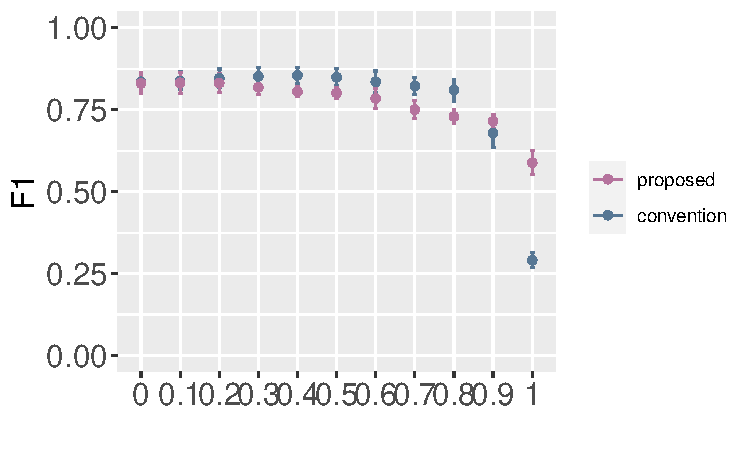
\includegraphics[scale=0.8]{graphics/f1_combined.pdf}
    \caption{\textbf{SCE was the stronger predictor of cancer prediction}. I combined GLE and SCE using two approaches: the conventional approach (bin for GLE and semi-symmetric 3-mer for SCE) and the proposed approach (smooth for GLE and asymmetric 3-mer for SCE). I used Euclidean distance for GLE and Jensen-Shannon distance for SCE. The x-axis is the weight given to GLE $g$, the weight given to SCE is accordingly $1-g$. For each weight combination, I iterated the training procedures 10 times. The y-axis is the means of $F1$ for all representations, the error bars are the standard errors for the iterated $F1$'s.}
    \label{fig:f1_combined}
\end{figure}
